\documentclass[11pt,letterpaper]{article}
\usepackage[top=2.0cm, bottom=3cm, left=2.0cm, right=2.0cm]{geometry}
\usepackage[utf8]{inputenc}
\usepackage[T1]{fontenc}
\usepackage[spanish]{varioref}
\usepackage[activeacute, spanish, es-tabla]{babel}
\usepackage{fancyhdr}
\usepackage{multicol}
\usepackage{float}
\usepackage{textcomp}
\usepackage{ae,aecompl}
\usepackage{amssymb,amsmath}
\usepackage[pdftex]{graphicx}
\pagestyle{fancy} 
\pagenumbering{arabic} 
\renewcommand{\headrulewidth}{0pt} 
\setlength{\headsep}{20pt} 
\setlength{\headheight}{65pt} 
\setlength{\textheight}{600pt} 
\setlength{\columnsep}{15pt} 
\newcommand{\universidad}{\small{Universidad Técnica Federico Santa María}}
\newcommand{\campus}{\small{Campus Santiago San Joaquín}}
\newcommand{\semestre}{\small{Segundo Semestre 2016}}

% Definiciones de Título e Integrantes de Experiencia
\newcommand{\titulo}{Tarea 4 - TALF}
\newcommand{\integrantes}{\begin{tabular}{c}
Jorge Contreras 201573547-6 \\
Juan Pablo Jorquera  201573533-6 \\
\end{tabular}}

\renewcommand{\maketitle}
{
\thispagestyle{fancy}
\begin{center}
\begin{Large}
\textbf{\titulo}\\
\end{Large}
\vspace{0.5cm}
\integrantes
\end{center}
\vspace{0.3cm}
}


%ENCABEZADO

\fancyhead[R]{\begin{minipage}[b]{0.405\textwidth}
\begin{center}
\universidad \\ 
\campus \\ 
\lab \\ 
\semestre
\end{center}
\end{minipage}}
\fancyhead[L]{\vspace{15pt}
\includegraphics[height=1.6cm]{Escudo.png}}
%%%%%%%%%%%%%%%%%%%%%%%%%%%%%%%%%%%%%%%%%%%%%%%%
%                                              %
% AQUI TERMINAN LAS DEFINICIONES DE ENCABEZADO %
% Y EMPIEZA EL CUERPO DEL DOCUMENTO            %
%                                              %
%%%%%%%%%%%%%%%%%%%%%%%%%%%%%%%%%%%%%%%%%%%%%%%%

\begin{document}
\maketitle

\section{Pregunta 1}
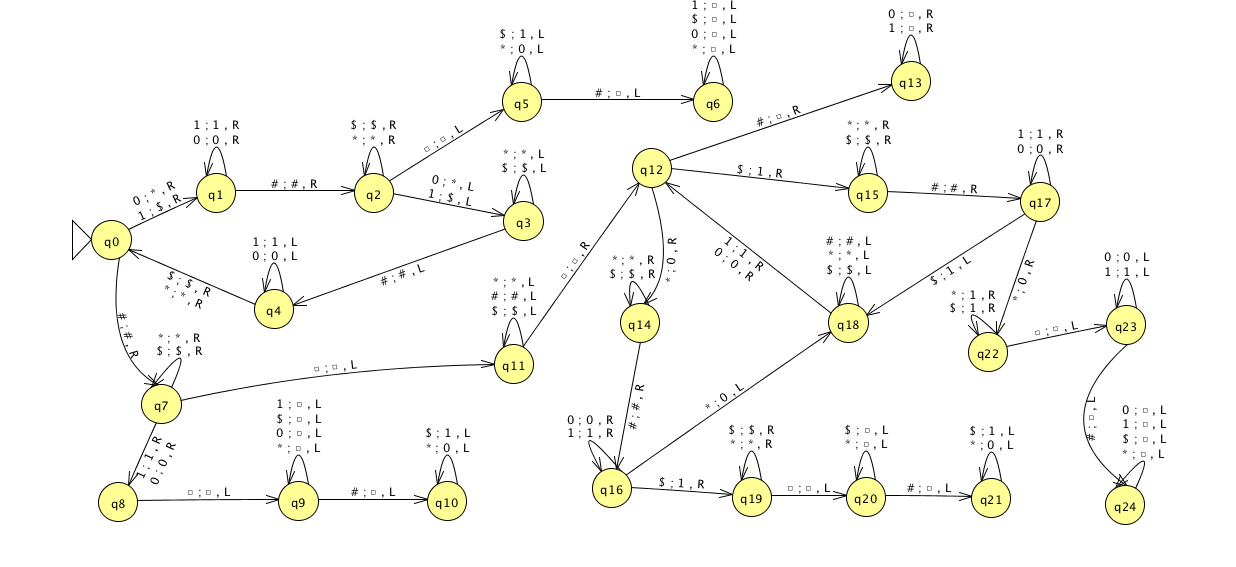
\includegraphics[height=8cm]{p1.png}
La máquina de Turing se divide en dos grandes partes: inicialmente compara los tamaños para decidir cual es el menor y luego, de ser iguales compara término a término para definir el menor.
\begin{itemize}
	\item Entre q0 y q4 va marcando los 1 con \$ y los 0 con \* y luego verifica que exista ese dígito en el término de la derecha.
	\item En q2 se sale al haber encontrado un dígito a la izquierda y haber terminado por completo el de la derecha, entonces el de la derecha es más corto, y en q5 y q6 lo decodifica y limpia el resto.
	\item En q0 se sale al haber terminado el primer término, entonces avanza hasta la posición actual del término de la derecha y verifica si también terminó.
	\item En caso de no haber terminado significa que el término de la izquierda era menor, entonces en q8, q9 y q10, limpia el término de la derecha y decodifica el de la izquierda.
	\item Por otro lado si también termina el término de la derecha, significa que eran de igual tamaño, donde avanza a q11 y de aquí se devuelve al comienzo de la cinta.
	\item Acá para comparar son dos partes virtualmente simétricas, dependiendo si comienza con 0 o 1 (codificado), lo decodifica y avanza al término de la derecha para comparar hasta q16 y q17 respectivamente.
	\item En caso de encontrar el mismo valor, se devuelve a q12 para seguir comparando.
	\item De no ser así se sale en q19 y q22 para terminar devolviendo el término adecuado en el resto de los nodos de esta rama.
	\item Finalmente en la situación de que ambos sean completamente iguales, se sale de q12 a q13, estándo ya decodificados por el loop los términos, simplemente borra el de la derecha.
\end{itemize}

\section{Pregunta 2}
S $\rightarrow$ bS | Sa | aSb | $\varepsilon$ \\
 \\
 
\noindent (a) Primero, aseamos la gramática \\
\indent S_{o} $\rightarrow$ S | $\varepsilon$ \\
\indent S $\rightarrow$ bS | Sa | aSb | b | a | ab \\

Luego, lo dejamos en FNC \\
\indent S_{o} $\rightarrow$ S | $\varepsilon$ \\
\indent S $\rightarrow$ BS | SA | XB | b | a | AB \\
\indent A $\rightarrow$ a \\
\indent B $\rightarrow$ b \\
\indent X $\rightarrow$ AS \\
 \\

 
\noindent (b) Palabra: aaa \\
\indent a$\hspace{2cm}$a$\hspace{2cm}$a \\
\indent $\downarrow$ $\hspace{1.7cm}$ $\downarrow$ $\hspace{1.75cm}$ $\downarrow$ \\
\indent S,A$\hspace{1.4cm}$S,A$\hspace{1.6cm}$S,A \\
 \\
\indent aa$\hspace{2cm}$aa \\
\indent $\downarrow$ $\hspace{2cm}$ $\downarrow$ \\
\indent S,X$\hspace{1.7cm}$S,X \\
 \\
\indent $\hspace{1cm}$aaa \\
\indent $\hspace{0.3cm}$ $\swarrow$ $\hspace{0.7cm}$ $\searrow$ \\
\indent a/aa$\hspace{1cm}$aa/a \\
\indent $\downarrow$ $\hspace{1.6cm}$ $\downarrow$ \\
\indent X$\hspace{1.75cm}$S \\
 \\
\indent aaa es formado por S y X, y por lo tanto pertenece a la gramática.
 \\
 \\
 \\
 
Palabra: bbaa \\ 
\indent b$\hspace{2cm}$b$\hspace{2cm}$a$\hspace{2cm}$a \\
\indent $\downarrow$ $\hspace{1.8cm}$ $\downarrow$ $\hspace{1.7cm}$ $\downarrow$ $\hspace{1.8cm}$ $\downarrow$ \\
\indent S,B$\hspace{1.5cm}$S,B$\hspace{1.6cm}$S,A$\hspace{1.6cm}$S,A \\
 \\
\indent bb$\hspace{2cm}$ba$\hspace{2cm}$aa \\
\indent $\downarrow$ $\hspace{2cm}$ $\downarrow$ $\hspace{2cm}$ $\downarrow$ \\
\indent S$\hspace{2.2cm}$S$\hspace{2.1cm}$S,X \\
 \\
\indent $\hspace{1cm}$bba$\hspace{4cm}$baa \\
\indent $\hspace{0.3cm}$ $\swarrow$ $\hspace{0.7cm}$ $\searrow$ $\hspace{2.7cm}$ $\swarrow$ $\hspace{0.7cm}$ $\searrow$ \\
\indent b/ba$\hspace{1cm}$bb/a $\hspace{1.8cm}$ b/aa$\hspace{1cm}$ba/a \\
\indent $\downarrow$ $\hspace{1.6cm}$ $\downarrow$ $\hspace{2.4cm}$ $\downarrow$ $\hspace{1.5cm}$ $\downarrow$ \\
\indent S$\hspace{1.75cm}$S $\hspace{2.4cm}$ S$\hspace{1.75cm}$S \\
 \\
\indent $\hspace{2.1cm}$bbaa \\
\indent $\hspace{1cm}$ $\swarrow$ $\hspace{0.6cm}$ $\downarrow$ $\hspace{0.7cm}$ $\searrow$ \\
\indent b/baa$\hspace{1cm}$bb/aa$\hspace{1cm}$bba/a \\
\indent $\hspace{0.3cm}$ $\downarrow$ $\hspace{1.5cm}$ $\downarrow$ $\hspace{1.6cm}$ $\downarrow$ \\
\indent $\hspace{0.4cm}$S$\hspace{1.6cm}$ $\emptyset$ $\hspace{1.8cm}$S \\
 \\
\indent bbaa es formado por S, por lo tanto pertenece a la gramática.
 \\
 \\
 \\
 
Palabra: aabba \\
\indent a$\hspace{2cm}$a$\hspace{2cm}$b$\hspace{2cm}$b$\hspace{2cm}$a \\
\indent $\downarrow$ $\hspace{1.8cm}$ $\downarrow$ $\hspace{1.7cm}$ $\downarrow$ $\hspace{1.8cm}$ $\downarrow$ $\hspace{1.8cm}$ $\downarrow$ \\
\indent S,A$\hspace{1.5cm}$S,A$\hspace{1.6cm}$S,B$\hspace{1.6cm}$S,B$\hspace{1.6cm}$S,A \\
 \\
\indent aa$\hspace{2cm}$ab$\hspace{2cm}$bb$\hspace{2cm}$ba \\
\indent $\downarrow$ $\hspace{2cm}$ $\downarrow$ $\hspace{2cm}$ $\downarrow$ $\hspace{2cm}$ $\downarrow$ \\
\indent S,X$\hspace{1.7cm}$S,X$\hspace{2cm}$S$\hspace{2.2cm}$S \\
 \\
\indent $\hspace{1cm}$aab$\hspace{4cm}$abb$\hspace{4.1cm}$bba \\
\indent $\hspace{0.3cm}$ $\swarrow$ $\hspace{0.7cm}$ $\searrow$ $\hspace{2.7cm}$ $\swarrow$ $\hspace{0.7cm}$ $\searrow$ $\hspace{2.7cm}$ $\swarrow$ $\hspace{0.7cm}$ $\searrow$ \\
\indent a/ab$\hspace{1cm}$aa/b $\hspace{1.8cm}$ a/bb$\hspace{1cm}$ab/b $\hspace{1.8cm}$ b/ba$\hspace{1cm}$bb/a \\
\indent $\downarrow$ $\hspace{1.6cm}$ $\downarrow$ $\hspace{2.4cm}$ $\downarrow$ $\hspace{1.5cm}$ $\downarrow$ $\hspace{2.4cm}$ $\downarrow$ $\hspace{1.5cm}$ $\downarrow$ \\
\indent X$\hspace{1.75cm}$S $\hspace{2.3cm}$ X$\hspace{1.75cm}$S $\hspace{2.3cm}$ S$\hspace{1.75cm}$S \\
 \\
\indent $\hspace{2.1cm}$aabb$\hspace{5.3cm}$abba \\
\indent $\hspace{1cm}$ $\swarrow$ $\hspace{0.6cm}$ $\downarrow$ $\hspace{0.7cm}$ $\searrow$ $\hspace{2cm}$ $\hspace{1cm}$ $\swarrow$ $\hspace{0.6cm}$ $\downarrow$ $\hspace{0.7cm}$ $\searrow$ \\
\indent a/abb$\hspace{1cm}$aa/bb$\hspace{1cm}$aab/b $\hspace{1cm}$ a/bba$\hspace{0.9cm}$ab/ba$\hspace{0.8cm}$abb/a \\
\indent $\hspace{0.3cm}$ $\downarrow$ $\hspace{1.5cm}$ $\downarrow$ $\hspace{1.6cm}$ $\downarrow$ $\hspace{1.7cm}$ $\downarrow$ $\hspace{1.5cm}$ $\downarrow$ $\hspace{1.5cm}$ $\downarrow$ \\
\indent $\hspace{0.4cm}$X$\hspace{1.6cm}$ $\emptyset$ $\hspace{1.7cm}$S $\hspace{1.6cm}$ X$\hspace{1.6cm}$ $\emptyset$ $\hspace{1.6cm}$S \\
 \\
\indent $\hspace{3.4cm}$aabba \\
\indent $\hspace{0.8cm}$ $\swarrow$ $\hspace{1.2cm}$ $\swarrow$ $\hspace{1.2cm}$ $\searrow$ $\hspace{1.2cm}$ $\searrow$ \\
\indent a/abba$\hspace{1cm}$aa/bba$\hspace{1cm}$aab/ba$\hspace{1cm}$aabb/a \\
\indent $\hspace{0.6cm}$ $\downarrow$ $\hspace{1.5cm}$ $\downarrow$ $\hspace{1.8cm}$ $\downarrow$ $\hspace{1.6cm}$ $\downarrow$ \\
\indent $\hspace{0.6cm}$X$\hspace{1.7cm}$ $\emptyset$ $\hspace{1.8cm}$ $\emptyset$ $\hspace{1.7cm}$S \\
 \\
\indent aabba es formado por S y X, por lo tanto pertenece a la gramática.
 \\

\noindent (c) El lenguaje acepta la palabra vacía y cualquier otra combinación que se pueda formar con las letras a y b.

\section{Pregunta 3}
$WHAT!?!?!?$


\section{Pregunta 4}
\subsection{Parte a}
Elijamos $w = a^{n^2}b^nc^n$ $\epsilon L_{1}$, con $|vy|>0$ y $|vxy|<n$ \\
Sea w de la forma w = uvxyz, al bombear encontramos con 5 casos: \\
1) $"u"$ e $"y"$ se encuentren dentro de $a^{n^2}$. \\
2) $"u"$ e $"y"$ se encuentren dentro de $b^n$. \\
3) $"u"$ e $"y"$ se encuentren dentro de $c^n$. \\
4) $"u"$ e $"y"$ se encuentren en la intersección de $a^{n^2}$ y $b^n$. \\
5) $"u"$ e $"y"$ se encuentren en la intersección de $b^n$ y $c^n$. \\
 \\
Bombeamos por casos. \\
 \\
1) uvxyz se encuentran dentro de $a^{n^2}$. \\
\indent $u=a^p$ \\
\indent $v=a^q$ \\
\indent $x=a^r$ \\
\indent $y=a^s$ \\
\indent $z=a^{n^2-p-q-r-s}b^nc^n$ \\
 \\
\indent k veces $"v"$ e $"y"$, quedando: \\
\indent $a^{n^2+(q+s)(k-1)}b^nc^n$ \\
\indent eligiendo k=2 \\
\indent $a^{n^2+(q+s)}b^nc^n$ \\
 \\
\indent Para que pertenesca al lenguaje, \\
\indent $n^2+q+s$ = n*n \\
\indent (q+s) = 0 \\
\indent Pero |vy|>0, existiendo así una contradicción. \\
 \\
2)Similar al caso 1, sólo que esta vez se bombea $b^n$, aumentando la cantidad de estas, quedando: \\
\indent $a^{n^2}b^{n+k}c^n$ \\
\indent con cualquier k>1 nos escapamos del lenguaje. \\
 \\
3)Simétrico al caso 2, sólo que esta vez se bombea $c^n$. \\
 \\
4)$"x"$ e $"y"$ se encontrarán dentro de las a's y las b's, quedando algo del estilo: \\
\indent $a^{n^2+k}b^{n+k}c^n$ \\
\indent bombeando hacia arriba con k=2 queda: \\
\indent $a^{n^2+2}b^{n+2}c^n$ \\
\indent Como no se cumple la igualdad, nos escapamos del lenguaje. \\
 \\
5)$"x"$ e $"y"$ se encontrarán dentro de las b's y las c's, quedando algo del estilo: \\
\indent $a^{n^2}b^{n+k}c^{n+k}$ \\
\indent bombeando hacia arriba con k=2 queda: \\
\indent $a^{n^2}b^{n+2}c^{n+2}$ \\
\indent Como no se cumple la igualdad, nos escapamos del lenguaje. \\

\noindent Como nos escapamos en todos los casos posibles, $L_{1}$ no es LLC

\subsection{Parte b}
	Primero vemos la ecuación de la forma $n = 8 - \frac{5}{3} m$, donde notamos que en los enteros no negativos solo hay dos combinaciones posibles:
	\begin{itemize}
		\item $m=0$; $n=8$
		\item $m=3$; $n=3$
	\end{itemize}
	Por lo que a continuación solo basta hacer el autómata correspondiente:
	\begin{center}
	\includegraphics[height=5cm]{4b.png}
	\end{center}
	Acá verificamos que incluso el lenguaje es regular, por lo que es de libre contexto.
\subsection{Parte c}
	Al igual que antes, es más fácil armar el PDA viendo la ecución de otra forma: $5m = 24 + 3n$
	\begin{center}
	\includegraphics[height=5.5cm]{4c.png}
	\end{center}
	Como hay PDA que lo represente, entonces es LLC.
\subsection{Parte d}
	A continuación se muestra el PDA del lenguaje, y como tiene PDA, entonces es LLC.
	\begin{center}
	\includegraphics[height=5.5cm]{4d.png}
	\end{center}


\subsection{Parte e}
Elijamos $w = a^nb^nca^nb^n$ $\epsilon L_{5}$, con $|vy|>0$ y $|vxy|<n$ \\
Sea w de la forma w = uvxyz, al bombear nos encontramos con 7 casos: \\
1) $"u"$ e $"y"$ se encuentren dentro de las primera $a^n$. \\
2) $"u"$ e $"y"$ se encuentren dentro de las segundas $a^n$. \\
3) $"u"$ e $"y"$ se encuentren dentro de las primeras $b^n$. \\
4) $"u"$ e $"y"$ se encuentren dentro de las segundas $b^n$. \\
5) $"u"$ e $"y"$ se encuentren en la primera intersección de a's y b's. \\
6) $"u"$ e $"y"$ se encuentren en la segunda intersección de a's y b's. \\
7) $"u"$ e $"y"$ se encuentren en la intersección de las $a^n$ con la c. \\
 \\
Bombeamos por casos. \\
 \\
1) uvxyz se encuentran dentro de $a^n$. \\
\indent $u=a^p$ \\
\indent $v=a^q$ \\
\indent $x=a^r$ \\
\indent $y=a^s$ \\
\indent $z=a^{n-p-q-r-s}b^nca^nb^n$ \\
 \\
\indent k veces $"v"$ e $"y"$, quedando: \\
\indent $a^{n+(q+s)(k-1)}b^nca^nb^n$ \\
\indent eligiendo k=0 \\
\indent $a^{n-q-s}b^nca^nb^n$ \\
 \\
\indent Para que pertenesca al lenguaje, \\
\indent n-q-s+n = n+n \\
\indent -(q+s) = 0 \\
\indent Pero |vy|>0, existiendo así una contradicción. \\
 \\
2) Simétrico al caso 1, sólo que esta vez se bombea las segundas $a^n$. \\
 \\
3) Simétrico al caso 1, sólo que esta vez se bombean las primeras $b^n$. \\
 \\
4) Simétrico al caso 1, sólo que esta vez se bombean las segundas $b^n$. \\
 \\
5) |vxy| se encuentra entre $a^nb^n$, siguiendo la lógica del caso 1) es evidente que si bombeamos hacia arriba aumentamos los valores de a y b, y no se cumpliría la igualdad, ya que los primeros a's y b's son más que los segundos, escapando así del lenguaje. \\
 \\
6) Simétrico al caso 5, sólo que esta vez se bombean las segundas $a^nb^n$. \\
 \\
7) En los casos en que c se encuentre dentro de $"v"$ o $"y"$ es evidente que al bombear hacia arriba va a aumentar la cantidad de c en la palabra y se escapa logicamente del lenguaje, entonces el caso a analizar es cuando c se encuentra en x. \\
 \\
\indent Así, si bombeamos hacia abajo, se eliminan las b's anteriores a c y las a's seguidas a c. \\
\indent $a^nb^{n-k}ca^{n-k}b^n$ \\
\indent k<0 nos escapamos del lenguaje. \\

\noindent Como nos escapamos en todos los casos posibles, $L_{5}$ no es LLC
  
\section{Pregunta 5}
\subsection{Parte a}
	\begin{itemize}
		\item Convertir GLC G en autómata de pila y expresión regular R en AFD.
		\item Construir PDA que incluya a G y a R simultáneamente ($L(G) \cap L(R)$), aceptando sólo en caso de que ambos acepten.
		\item Transformar nuevo PDA a GLC.
		\item Aplicar CYK sobre dicho GLC para verificar la pertenencia.
	\end{itemize}
\subsection{Parte b}
	\begin{itemize}
		\item Realizar aseo sobre GLC.
		\item En el GLC verificar si existe algún loop, es decir, si alguna variable se produce a sí misma, o bien se producen entre ellas. De ser así inmediatamente se sabe que existe una palabra $w$ tal que $|w| \geq n$.
		\item Realizar árbol sobre la gramática con S en la raíz, poninendo en los hijos todas las opciones de variables.
		\item Repetir el paso anterior para cada hijo incluyendo las combinaciones posibles en cada una.
		\item En caso de encontrar alguno de los hijos con largo mayor a $n$, entonces dicha palabra existe. Por otro lado, si se terminó el árbol y no se encontró, entonces dicho lenguaje no contiene palabras con dichas características.
	\end{itemize}

\end{document}
